\chapter{Energi Reaksi: Pembakaran dan Energi Ikatan}\label{ch:g11:reaction-energy}

Robeklah segel sebuah penghangat tangan dan, semenit kemudian, benda itu
terlalu panas untuk digenggam lama; remaslah sebuah kantong dingin
instan dan kantong itu mendinginkan pergelangan kaki yang terkilir;
sebuah bus kota berjalan seharian dengan hidrogen dan hanya meninggalkan
uap air di belakangnya. \omterm{def:g5:irreversible-changes:chemical-change}{Perubahan kimia} tidak hanya mengubah zat menjadi
zat lain: perubahan itu melepaskan energi, atau menyerapnya. Dari mana
energi itu berasal, dan berapa banyak yang dapat diberikan sebuah \omterm{def:g4:what-a-fire-needs:fuel}{bahan
bakar}?

\begin{recall}
Dalam \omterm{def:g8:combustion-and-fuels:complete}{pembakaran sempurna}, \omterm{def:g4:what-a-fire-needs:fuel}{bahan bakar} yang tersusun atas karbon dan
hidrogen \omterm{def:g4:what-a-fire-needs:burning}{terbakar} dalam oksigen dan menghasilkan karbon dioksida dan air
(\cref{ch:g8:combustion-and-fuels}). \omterm{def:g10:lewis-and-shape:covalent-bond}{Ikatan kovalen} adalah pasangan
\omterm{def:g9:inside-the-atom:nucleus}{elektron} yang dipakai bersama; \omterm{def:g10:lewis-and-shape:lewis-structure}{struktur Lewis} memperlihatkan setiap
ikatan dalam sebuah \omterm{def:g7:atoms-and-molecules:molecule}{molekul} (\cref{ch:g10:lewis-and-shape}). \omterm{def:g10:the-mole:amount}{Jumlah zat}
dihitung dalam \omterm{def:g10:the-mole:amount}{mol} (\cref{ch:g10:the-mole}).
\end{recall}

\begin{omfigure}
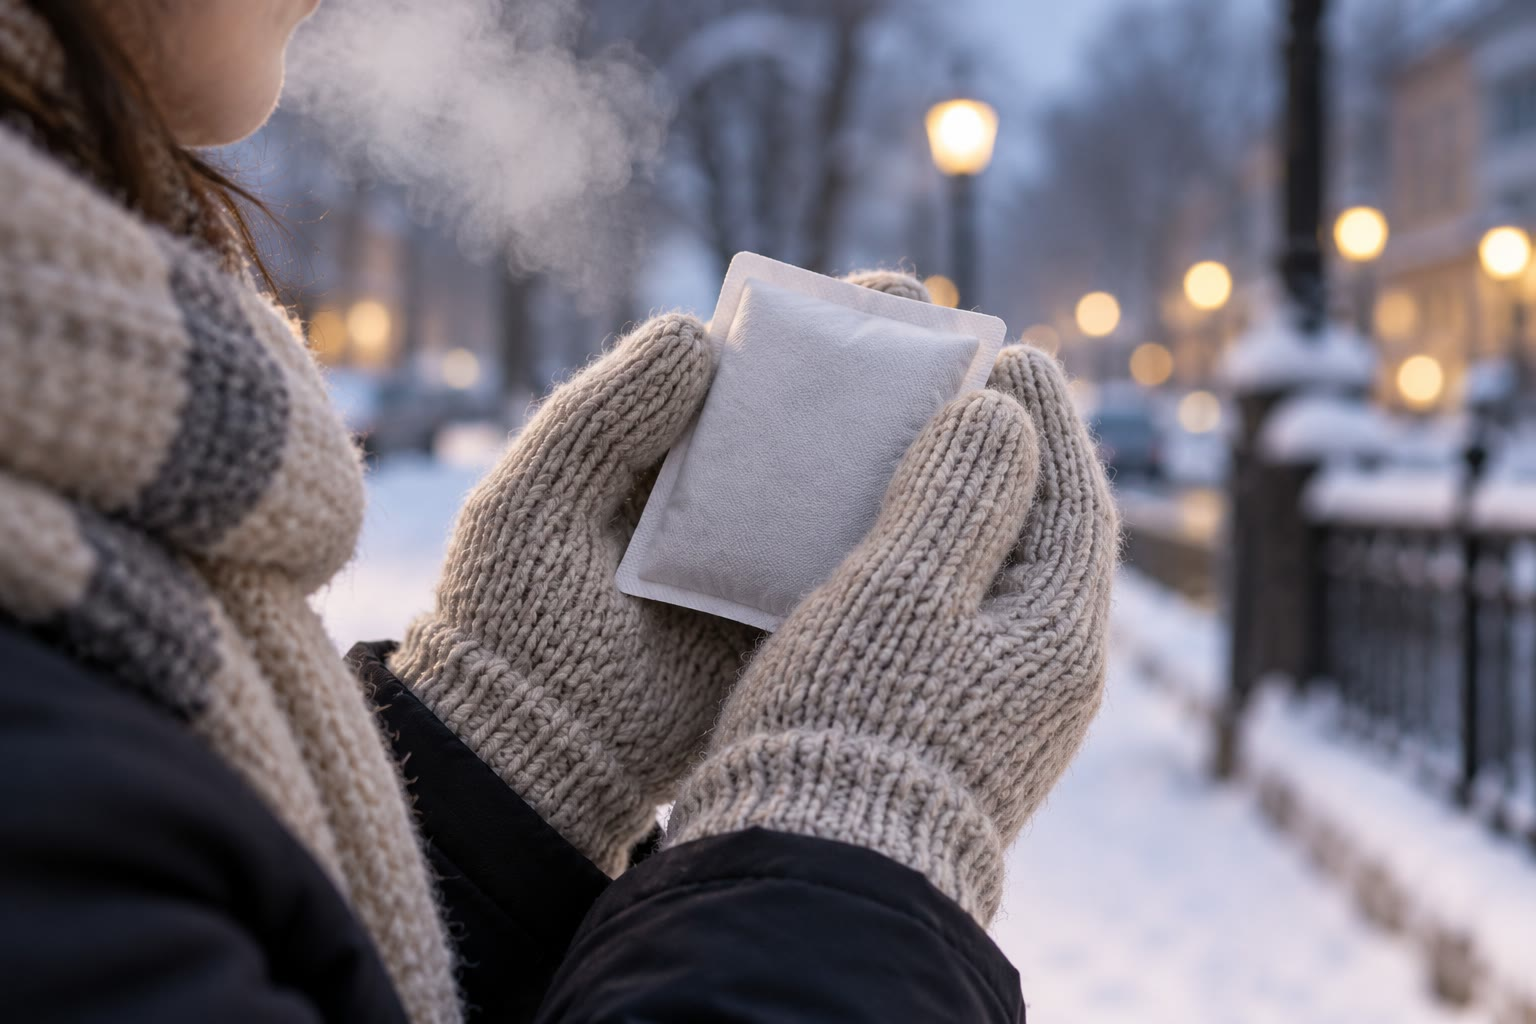
\includegraphics[width=0.45\linewidth]{images/book1/ai/g11-hand-warmers.jpg}

{\small Penghangat tangan: sebuah reaksi di dalam kantongnya melepaskan
panas.}
\end{omfigure}

\section{Perubahan eksoterm dan endoterm}

\begin{definition}[Eksoterm, endoterm]\label{def:g11:reaction-energy:exothermic}
Sebuah perubahan disebut \emph{eksoterm}\index{eksoterm} jika perubahan
itu melepaskan energi ke lingkungannya, biasanya sebagai panas:
lingkungannya menjadi hangat. Perubahan itu disebut
\emph{endoterm}\index{endoterm} jika menyerap energi dari lingkungannya:
lingkungannya menjadi dingin, atau perubahan itu perlu dipanaskan agar
terus berlangsung.
\end{definition}

\begin{example}[Hangat dan dingin]\label{ex:g11:reaction-energy:packs}
\omterm{def:g4:what-a-fire-needs:burning}{Pembakaran} bersifat \omterm{def:g11:reaction-energy:exothermic}{eksoterm}, demikian pula reaksi lambat serbuk besi
dengan oksigen \omterm{def:g4:air-a-mixture-of-gases:air}{udara} di dalam penghangat tangan. Pelarutan amonium
nitrat dalam air, yang dipakai dalam kantong dingin instan, bersifat
\omterm{def:g11:reaction-energy:exothermic}{endoterm}; demikian pula penguraian batu kapur menjadi kapur tohor dan
karbon dioksida, yang hanya berlangsung di dalam tanur yang sangat
panas.
\end{example}

\begin{omfigure}
\begin{tikzpicture}[font=\small]
  \begin{scope}
    \draw[->] (0,0) -- (0,3.2) node[above] {energi};
    \draw[very thick, omDef] (0.5,2.5) -- (2.3,2.5) node[right, text=black] {pereaksi};
    \draw[very thick, omProp] (0.5,0.8) -- (2.3,0.8) node[right, text=black] {produk};
    \draw[->, thick, omThm] (1.4,2.45) -- (1.4,0.85);
    \node[omThm, anchor=west, align=left] at (1.5,1.65) {energi\\ dilepaskan};
    \node[anchor=north] at (1.6,-0.15) {\textbf{eksoterm}};
  \end{scope}
  \begin{scope}[xshift=6cm]
    \draw[->] (0,0) -- (0,3.2) node[above] {energi};
    \draw[very thick, omDef] (0.5,0.8) -- (2.3,0.8) node[right, text=black] {pereaksi};
    \draw[very thick, omProp] (0.5,2.5) -- (2.3,2.5) node[right, text=black] {produk};
    \draw[->, thick, omDef] (1.4,0.85) -- (1.4,2.45);
    \node[omDef, anchor=west, align=left] at (1.5,1.65) {energi\\ diserap};
    \node[anchor=north] at (1.6,-0.15) {\textbf{endoterm}};
  \end{scope}
\end{tikzpicture}

{\small Diagram energi. Dalam reaksi \omterm{def:g11:reaction-energy:exothermic}{eksoterm}, produk menyimpan energi
lebih sedikit daripada \omterm{def:g7:chemical-reactions:reactant}{pereaksi}, dan selisihnya dilepaskan; dalam reaksi
\omterm{def:g11:reaction-energy:exothermic}{endoterm}, produk menyimpan lebih banyak, dan selisihnya harus diberikan.}
\end{omfigure}

\section{Energi yang dilepaskan pembakaran}

\begin{definition}[Energi pembakaran molar]\label{def:g11:reaction-energy:combustion-energy}
Yang disebut \emph{energi pembakaran molar}\index{energi pembakaran molar}
$E_c$ sebuah \omterm{def:g4:what-a-fire-needs:fuel}{bahan bakar} adalah energi yang dilepaskan oleh \omterm{def:g8:combustion-and-fuels:complete}{pembakaran
sempurna} satu \omterm{def:g10:the-mole:amount}{mol} \omterm{def:g4:what-a-fire-needs:fuel}{bahan bakar} itu, dalam \si{kJ/mol}, dengan air yang
terbentuk berwujud cair.
\end{definition}

\begin{proposition}[Energi yang dilepaskan $n$ mol]\label{prop:g11:reaction-energy:n-moles}
% ledger: dch:CH4
\omterm{def:g8:combustion-and-fuels:complete}{Pembakaran sempurna} \omterm{def:g4:what-a-fire-needs:fuel}{bahan bakar} sejumlah $n$ melepaskan energi
$Q = n \times E_c$. Untuk metana, $E_c = \qty{890.7}{kJ/mol}$: membakar
\qty{1.00}{mol} (\qty{16.0}{g}) metana melepaskan sekitar \qty{891}{kJ}.
\end{proposition}

\begin{proof}
Setiap \omterm{def:g10:the-mole:amount}{mol} \omterm{def:g4:what-a-fire-needs:fuel}{bahan bakar} yang \omterm{def:g4:what-a-fire-needs:burning}{terbakar} melepaskan $E_c$; $n$ \omterm{def:g10:the-mole:amount}{mol}
melepaskan $n$ kali lebih banyak.
\end{proof}

\begin{inthelab}[Memanaskan air dengan pembakar spiritus]
% ledger: cp:water
Sebuah pembakar spiritus berisi etanol ditimbang, lalu dinyalakan di
bawah kaleng \omterm{def:g9:periodic-table-first-look:metal}{logam} berisi \qty{200}{g} air yang diberi termometer.
Ketika suhu air telah naik \qty{25}{\celsius}, nyala api dipadamkan dan
pembakar ditimbang lagi: pembakar telah kehilangan \qty{1.50}{g} etanol.
Energi yang diterima air dihitung dengan rumus fisika
$Q = m\, c\, \Delta\theta$, dengan $c = \qty{4.18}{J/(g.\celsius)}$
kalor jenis air. Energi itu jauh di bawah energi yang dapat dilepaskan
etanolnya: sebagian besar panasnya menghangatkan \omterm{def:g4:air-a-mixture-of-gases:air}{udara}, kaleng, dan
pembakar, dan sebagian etanol \omterm{def:g4:what-a-fire-needs:burning}{terbakar} tidak sempurna.
\end{inthelab}

\begin{omfigure}
\begin{tikzpicture}[font=\small]
  % spirit burner
  \fill[black!8, draw=black!60] (-0.6,0) rectangle (0.6,0.7);
  \fill[cyan!15] (-0.55,0.05) rectangle (0.55,0.45);
  \fill[black!40] (-0.06,0.7) rectangle (0.06,0.95);
  \fill[orange!70!yellow] (0,0.95) .. controls (-0.25,1.25) and (-0.1,1.6) .. (0,1.85)
    .. controls (0.1,1.6) and (0.25,1.25) .. (0,0.95);
  \fill[yellow!40] (0,1.0) .. controls (-0.1,1.2) and (-0.05,1.4) .. (0,1.5)
    .. controls (0.05,1.4) and (0.1,1.2) .. (0,1.0);
  % tripod and can
  \draw[black!60, line width=1pt] (-1.1,0) -- (-0.9,2.1) (1.1,0) -- (0.9,2.1);
  \draw[black!60, line width=1.2pt] (-1.1,2.1) -- (1.1,2.1);
  \fill[black!15, draw=black!60] (-0.8,2.1) rectangle (0.8,3.7);
  \fill[omWater] (-0.75,2.15) rectangle (0.75,3.3);
  % thermometer
  \pic at (0.35,2.35) {thermometer};
  \draw[omProp, thick, <-] (0.6,0.35) -- (2.0,0.35) node[right, text=black]
    {pembakar spiritus (etanol)};
  \draw[omProp, thick, <-] (0.8,2.9) -- (2.0,2.9) node[right, text=black]
    {kaleng: \qty{200}{g} air};
  \draw[omProp, thick, <-] (0.45,5.0) -- (2.0,5.0) node[right, text=black]
    {termometer};
\end{tikzpicture}

{\small Mengukur energi yang diberikan sebuah \omterm{def:g4:what-a-fire-needs:fuel}{bahan bakar}: pembakar
spiritus memanaskan sekaleng air yang kenaikan suhunya diukur.}
\end{omfigure}


\begin{example}[Pembakar spiritus dalam angka]\label{ex:g11:reaction-energy:burner}
% ledger: cp:water, dch:C2H5OH, aw:C, aw:H, aw:O
Air menerima $Q = 200 \times 4.18 \times 25 = \qty{2.09e4}{J}$, yaitu
\qty{20.9}{kJ}. Etanol yang \omterm{def:g4:what-a-fire-needs:burning}{terbakar}, \qty{1.50}{g}, adalah
$1.50 / 46.0 = \qty{0.0326}{mol}$; dengan $E_c = \qty{1367.6}{kJ/mol}$
etanol itu dapat melepaskan $0.0326 \times 1367.6 = \qty{44.6}{kJ}$.
Hanya $20.9 / 44.6 \approx \qty{47}{\percent}$ darinya yang sampai ke
air.
\end{example}

\section{Energi ikatan}

\begin{definition}[Energi ikatan]\label{def:g11:reaction-energy:bond-energy}
Yang disebut \emph{energi ikatan}\index{energi ikatan} sebuah \omterm{def:g10:lewis-and-shape:covalent-bond}{ikatan
kovalen} adalah energi yang diperlukan untuk memutus satu \omterm{def:g10:the-mole:amount}{mol} ikatan
semacam itu, dengan \omterm{def:g7:atoms-and-molecules:molecule}{molekul} dan \omterm{def:g7:atoms-and-molecules:atom}{atomnya} berwujud gas. Tabel memberikan
nilai rata-rata, yang diukur pada banyak \omterm{def:g7:atoms-and-molecules:molecule}{molekul}, dalam \si{kJ/mol}.
\end{definition}

\begin{omfigure}
\small
% ledger: be:H-H, be:C-H, be:N-H, be:O-H, be:H-Cl, be:C-C, be:CC-double, be:C-O, be:CO-double, be:NN-triple, be:OO-double, be:Cl-Cl
\begin{tabular}{lr@{\qquad}lr@{\qquad}lr}
\hline
ikatan & \si{kJ/mol} & ikatan & \si{kJ/mol} & ikatan & \si{kJ/mol} \\
\hline
\ce{H-H} & 436 & \ce{C-C} & 345 & \ce{O=O} & 498 \\
\ce{C-H} & 415 & \ce{C=C} & 611 & \ce{N#N} & 946 \\
\ce{N-H} & 390 & \ce{C-O} & 350 & \ce{Cl-Cl} & 243 \\
\ce{O-H} & 464 & \ce{C=O} & 741 & \ce{H-Cl} & 432 \\
\hline
\end{tabular}\par\medskip

{\small \omterm{def:g11:reaction-energy:bond-energy}{Energi ikatan} rata-rata. Memutus ikatan selalu memerlukan
energi; membentuknya mengembalikan energi yang sama.}
\end{omfigure}

\begin{omfigure}
\begin{tikzpicture}[font=\small, x=1cm, y=0.0015cm]
  \draw[->] (0,-850) -- (0,2900) node[above] {energi (\si{kJ})};
  \draw[very thick, black!60] (0.4,2656) -- (3.9,2656);
  \node[anchor=west] at (4.0,2656) {atom-atom terpisah: \ce{C + 4H + 4O}};
  \draw[very thick, omDef] (0.4,0) -- (3.9,0);
  \node[anchor=west] at (4.0,0) {\ce{CH4 + 2O2}};
  \draw[very thick, omProp] (0.4,-682) -- (3.9,-682);
  \node[anchor=west] at (4.0,-682) {\ce{CO2 + 2H2O}};
  \draw[->, thick, omDef] (1.0,30) -- (1.0,2626);
  \node[omDef, anchor=west, align=left] at (1.05,1500) {memutus\\ 4 \ce{C-H} dan\\ 2 \ce{O=O}:\\ $+\qty{2656}{kJ}$};
  \draw[->, thick, omProp] (3.4,2626) -- (3.4,-652);
  \node[omProp, anchor=west, align=left] at (3.45,1200) {membentuk 2 \ce{C=O}\\ dan 4 \ce{O-H}:\\ $-\qty{3338}{kJ}$};
  \draw[<->, omThm, thick] (0.6,-10) -- (0.6,-672);
  \node[omThm, anchor=west] at (0.65,-341) {$E_r \approx \qty{-682}{kJ}$};
\end{tikzpicture}

{\small \omterm{def:g4:what-a-fire-needs:burning}{Pembakaran} metana sebagai dua tahap khayalan, dengan \omterm{def:g11:reaction-energy:bond-energy}{energi
ikatan} rata-rata: semua ikatan diputus, lalu ikatan-ikatan baru
terbentuk. Perkiraannya, \qty{-682}{kJ} per \omterm{def:g10:the-mole:amount}{mol} metana, bersifat
\omterm{def:g11:reaction-energy:exothermic}{eksoterm}.}
\end{omfigure}

\begin{proposition}[Memperkirakan energi reaksi]\label{prop:g11:reaction-energy:estimate}
Untuk reaksi antargas, energi yang diserap, $E_r$ (negatif jika energi
dilepaskan), kurang lebih
\[
  E_r \approx \sum E(\text{ikatan diputus}) - \sum E(\text{ikatan dibentuk}) .
\]
Jika $E_r < 0$, energi yang dilepaskan pembentukan ikatan-ikatan baru
lebih besar daripada energi yang diperlukan untuk memutus ikatan-ikatan
lama: reaksinya \omterm{def:g11:reaction-energy:exothermic}{eksoterm}.
\end{proposition}

\begin{proof}
Bayangkan reaksi itu dalam dua tahap: setiap ikatan \omterm{def:g7:chemical-reactions:reactant}{pereaksi} diputus,
yang memerlukan jumlah pertama dan menyisakan \omterm{def:g7:atoms-and-molecules:atom}{atom-atom} terpisah; lalu
ikatan-ikatan produk terbentuk, yang mengembalikan jumlah kedua.
Hasilnya hanya sebuah perkiraan, karena tabel memberikan nilai rata-rata
pada banyak \omterm{def:g7:atoms-and-molecules:molecule}{molekul}.
\end{proof}

\begin{method}[Memperkirakan energi reaksi dari energi ikatan]\label{met:g11:reaction-energy:bonds}
\begin{enumerate}
  \item Tuliskan \omterm{def:g8:balanced-equations:equation}{persamaan setaranya} dan \omterm{def:g10:lewis-and-shape:lewis-structure}{struktur Lewis} setiap \omterm{def:g7:atoms-and-molecules:molecule}{molekul}.
  \item Hitunglah ikatan setiap jenis yang diputus dalam \omterm{def:g7:chemical-reactions:reactant}{pereaksi} dan
        yang dibentuk dalam produk, dengan memperhitungkan koefisiennya.
  \item Jumlahkan \omterm{def:g11:reaction-energy:bond-energy}{energi ikatan} yang diputus, lalu kurangi dengan \omterm{def:g11:reaction-energy:bond-energy}{energi
        ikatan} yang dibentuk.
  \item Simpulkan: hasil negatif berarti reaksi \omterm{def:g11:reaction-energy:exothermic}{eksoterm}.
\end{enumerate}
\end{method}

\begin{example}[Hidrogen dan klorin]\label{ex:g11:reaction-energy:hcl}
% ledger: be:H-H, be:Cl-Cl, be:H-Cl
Untuk \ce{H2 + Cl2 -> 2HCl}: satu \ce{H-H} dan satu \ce{Cl-Cl} diputus,
$436 + 243 = \qty{679}{kJ}$; dua \ce{H-Cl} dibentuk, $2 \times 432 =
\qty{864}{kJ}$. Jadi $E_r \approx 679 - 864 = \qty{-185}{kJ}$ per \omterm{def:g10:the-mole:amount}{mol}
reaksi: \omterm{def:g11:reaction-energy:exothermic}{eksoterm}.
\end{example}


\begin{remark}[Perkiraan dan pengukuran]\label{rem:g11:reaction-energy:compare}
% ledger: dch:CH4
Energi terukur yang dilepaskan \omterm{def:g4:what-a-fire-needs:burning}{pembakaran} satu \omterm{def:g10:the-mole:amount}{mol} metana adalah
\qty{890.7}{kJ}, lebih besar daripada perkiraannya. Ada tiga alasan:
ikatan \ce{C=O} karbon dioksida lebih kuat daripada \ce{C=O} rata-rata
dalam tabel; nilai terukurnya berlaku untuk air cair, dan pengembunan
uap air melepaskan energi tambahan; dan \omterm{def:g11:reaction-energy:bond-energy}{energi ikatan} rata-rata
hanyalah rata-rata. Metode \omterm{def:g11:reaction-energy:bond-energy}{energi ikatan} memberikan tanda dan orde
besarnya, bukan nilai tepatnya.
\end{remark}

\section{Membandingkan bahan bakar}

\begin{omfigure}
\begin{tikzpicture}
\begin{axis}[xbar, width=0.78\linewidth, height=5.4cm, xmin=0, xmax=160,
    xlabel={energi yang dilepaskan per kilogram yang terbakar (\si{MJ/kg})},
    symbolic y coords={ethanol, octane, propane, methane, hydrogen},
    yticklabels={etanol, oktana, propana, metana, hidrogen},
    ytick=data, bar width=10pt, nodes near coords,
    nodes near coords style={font=\footnotesize, /pgf/number format/fixed,
      /pgf/number format/precision=1, /pgf/number format/fixed zerofill},
    tick label style={font=\small}, label style={font=\small},
    axis lines*=left, xmajorgrids, grid style={gray!20}, enlarge y limits=0.15]
  % ledger: dch:C2H5OH, dfh:C8H18, dfh:CO2, dfh:H2O-l, dch:C3H8, dch:CH4 (per kg with the book's molar masses)
  \addplot[fill=omProp!55, draw=omProp] coordinates {(29.7,ethanol) (48.0,octane)
    (50.4,propane) (55.7,methane) (142.9,hydrogen)};
\end{axis}
\end{tikzpicture}

{\small Energi yang dilepaskan oleh \omterm{def:g8:combustion-and-fuels:complete}{pembakaran sempurna} satu kilogram
lima \omterm{def:g4:what-a-fire-needs:fuel}{bahan bakar} (air yang terbentuk berwujud cair). Hidrogen memberikan
paling banyak per kilogram, jauh di atas yang lain; etanol, yang sudah
``setengah \omterm{def:g4:what-a-fire-needs:burning}{terbakar}'' (mengandung oksigen), paling sedikit.}
\end{omfigure}

\begin{example}[Karbon dioksida per megajoule]\label{ex:g11:reaction-energy:co2}
% ledger: dch:CH4, dch:C2H5OH
Membakar satu \omterm{def:g10:the-mole:amount}{mol} metana melepaskan \qty{890.7}{kJ} dan satu \omterm{def:g10:the-mole:amount}{mol} karbon
dioksida, \qty{44.0}{g}. Untuk satu megajoule, \qty{1000}{kJ}, metana
melepaskan $44.0 \times 1000 / 890.7 = \qty{49.4}{g}$ karbon dioksida.
Etanol, dengan dua \omterm{def:g10:the-mole:amount}{mol} karbon dioksida per \qty{1367.6}{kJ}, melepaskan
$88.0 \times 1000 / 1367.6 = \qty{64.3}{g}$ per megajoule. Hidrogen
tidak melepaskan karbon dioksida sama sekali: satu-satunya produknya
adalah air.
\end{example}

\begin{omfigure}
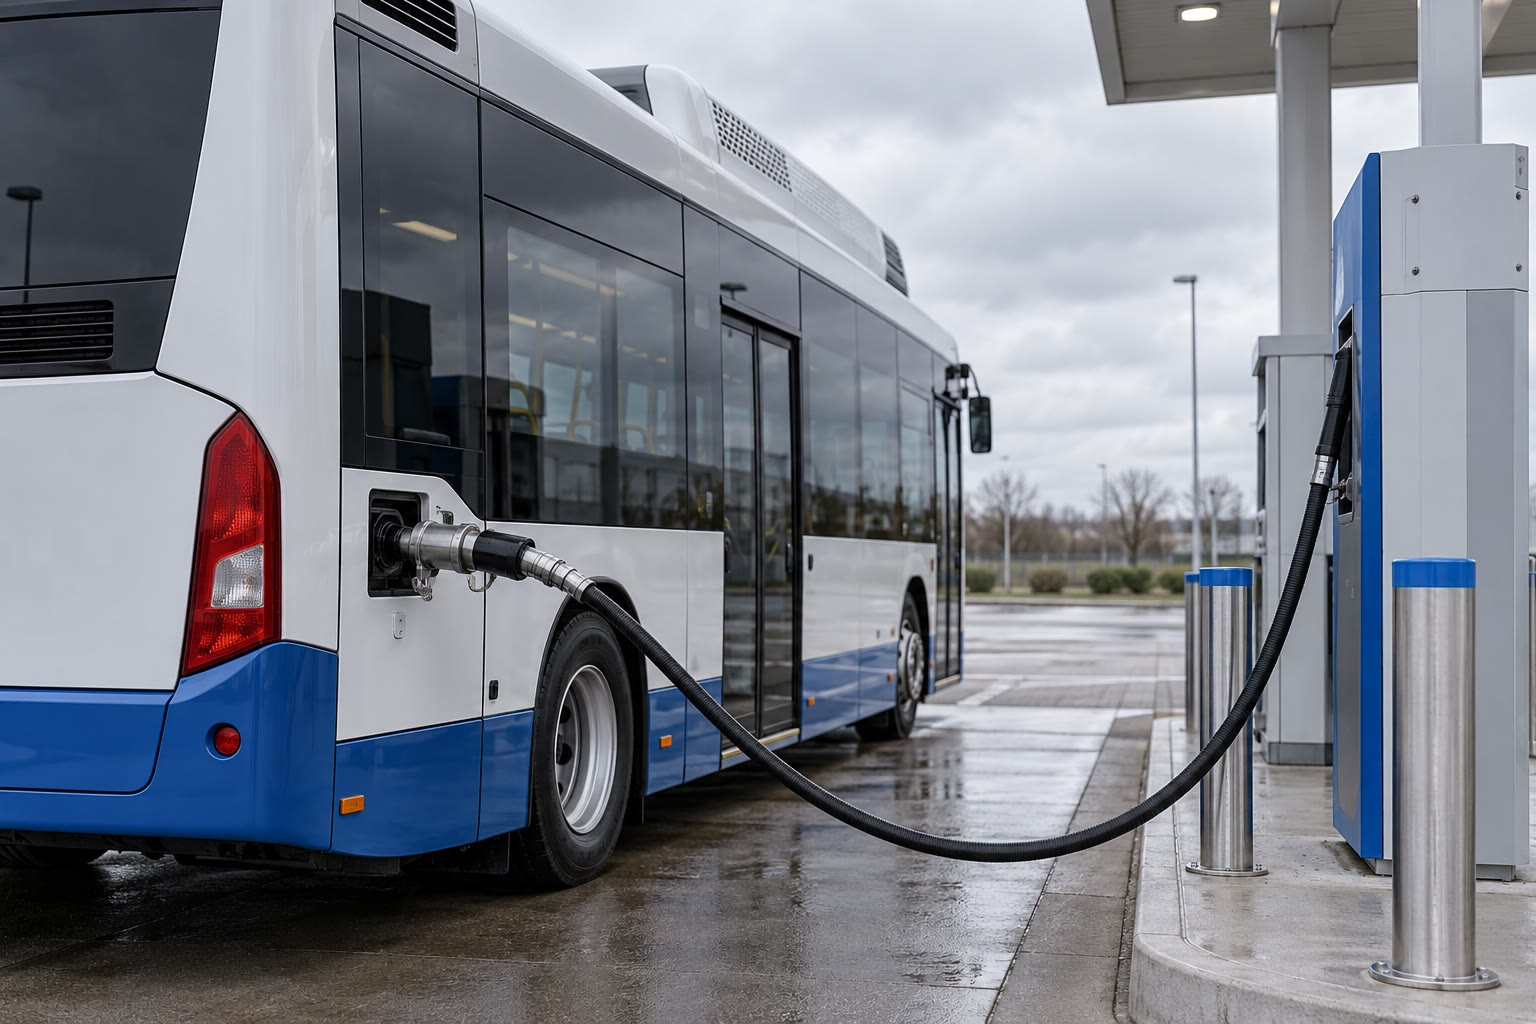
\includegraphics[width=0.5\linewidth]{images/book1/ai/g11-hydrogen-bus.jpg}

{\small Sebuah bus di stasiun pengisian hidrogen: \omterm{def:g4:what-a-fire-needs:fuel}{bahan bakarnya} hanya
melepaskan air.}
\end{omfigure}

\begin{safety}{\ghs[0.82cm]{GHS02}\ghs[0.82cm]{GHS07}}
% ledger: ghs:ethanol
Etanol sangat mudah menyala dan menyebabkan iritasi mata. Pembakar
spiritus diisi jauh dari nyala api, tidak pernah diisi ulang selagi
panas, dan dipakai oleh guru di atas alas tahan panas.
\end{safety}

\section{Latihan}


\begin{exercise}[$\star$]\label{exo:g11:reaction-energy:1}
\omterm{def:g11:reaction-energy:exothermic}{Eksoterm} atau \omterm{def:g11:reaction-energy:exothermic}{endoterm}: kayu yang \omterm{def:g4:what-a-fire-needs:burning}{terbakar}; es yang mencair; kantong
dingin instan yang diremas; penghangat tangan yang memanas; daun hijau
yang membuat gula di bawah sinar matahari?
\end{exercise}

\begin{exercise}[$\star$]\label{exo:g11:reaction-energy:2}
% ledger: dch:CH4
Berapa energi yang dilepaskan \omterm{def:g8:combustion-and-fuels:complete}{pembakaran sempurna} \qty{3.0}{mol}
metana?
\end{exercise}

\begin{exercise}[$\star$]\label{exo:g11:reaction-energy:3}
Pada diagram energi sebuah reaksi \omterm{def:g11:reaction-energy:exothermic}{eksoterm}, mana yang menyimpan energi
lebih banyak, \omterm{def:g7:chemical-reactions:reactant}{pereaksi} atau produk? Ke mana selisihnya pergi?
\end{exercise}

\begin{exercise}[$\star$]\label{exo:g11:reaction-energy:4}
% ledger: dch:C2H5OH
Berapa energi yang dilepaskan \omterm{def:g8:combustion-and-fuels:complete}{pembakaran sempurna} \qty{100}{g} etanol?
\end{exercise}

\begin{exercise}[$\star$]\label{exo:g11:reaction-energy:5}
Apa itu \omterm{def:g11:reaction-energy:bond-energy}{energi ikatan}? Mengapa memutus ikatan selalu memerlukan energi?
\end{exercise}

\begin{exercise}[$\star\star$]\label{exo:g11:reaction-energy:6}
Perkirakan, dengan \omterm{def:g11:reaction-energy:bond-energy}{energi ikatan}, energi reaksi
\ce{2H2 + O2 -> 2H2O}, semuanya gas. Apakah reaksi itu \omterm{def:g11:reaction-energy:exothermic}{eksoterm}?
\end{exercise}

\begin{exercise}[$\star\star$]\label{exo:g11:reaction-energy:7}
Perkirakan energi \omterm{def:g4:what-a-fire-needs:burning}{pembakaran} etanol, \ce{C2H5OH + 3O2 ->
2CO2 + 3H2O}, dengan \omterm{def:g11:reaction-energy:bond-energy}{energi ikatan} (gambarlah dahulu \omterm{def:g10:lewis-and-shape:lewis-structure}{struktur Lewis}
etanol), lalu bandingkan dengan nilai terukur \qty{1367.6}{kJ/mol}.
\end{exercise}

\begin{exercise}[$\star\star$]\label{exo:g11:reaction-energy:8}
% ledger: dch:C3H8, dch:CH4
Hitung energi yang dilepaskan per kilogram propana
(\qty{2219.2}{kJ/mol}) dan per kilogram metana. Bandingkan dengan
diagram batang.
\end{exercise}

\begin{exercise}[$\star\star$]\label{exo:g11:reaction-energy:9}
% ledger: cp:water, dch:CH4
Sebuah kompor gas memanaskan \qty{1.50}{L} air (\qty{1500}{g}) dari
\qty{15}{\celsius} sampai \qty{100}{\celsius}. Berapa energi yang
diterima air? Berapa massa metana yang \omterm{def:g4:what-a-fire-needs:burning}{terbakar} jika seluruh energinya
sampai ke air? Jika hanya setengahnya?
\end{exercise}

\begin{exercise}[$\star\star$]\label{exo:g11:reaction-energy:10}
Dengan diagram batang, urutkan \omterm{def:g4:what-a-fire-needs:fuel}{bahan bakar} menurut energinya per
kilogram. Berapa massa hidrogen yang memberikan energi yang sama dengan
\qty{1.0}{kg} oktana?
\end{exercise}

\begin{exercise}[$\star\star$]\label{exo:g11:reaction-energy:11}
Perkirakan energi reaksi \ce{N2 + 3H2 -> 2NH3}, semuanya gas. \omterm{def:g11:reaction-energy:exothermic}{Eksoterm}
atau \omterm{def:g11:reaction-energy:exothermic}{endoterm}?
\end{exercise}

\begin{exercise}[$\star\star\star$]\label{exo:g11:reaction-energy:12}
% ledger: cp:water, dch:C2H5OH
Dalam percobaan pembakar spiritus, suhu \qty{250}{g} air naik
\qty{20}{\celsius} sementara \qty{1.20}{g} etanol \omterm{def:g4:what-a-fire-needs:burning}{terbakar}. Hitung
energi yang diterima air, energi yang dapat dilepaskan etanol, dan
efisiensi pemanasannya. Sebutkan tiga penyebab kehilangan energinya.
\end{exercise}

\begin{exercise}[$\star\star\star$]\label{exo:g11:reaction-energy:13}
% ledger: dfh:C8H18, dfh:CO2, dfh:H2O-l, dch:C3H8
Oktana melepaskan \qty{5470}{kJ/mol} dan propana \qty{2219.2}{kJ/mol}.
Tuliskan persamaan \omterm{def:g4:what-a-fire-needs:burning}{pembakarannya}, lalu hitung massa karbon dioksida
yang dilepaskan masing-masing per megajoule. Bandingkan dengan metana,
\qty{49.4}{g}.
\end{exercise}

\begin{exercise}[$\star\star\star$]\label{exo:g11:reaction-energy:14}
Untuk metana maupun etanol, perkiraan dengan \omterm{def:g11:reaction-energy:bond-energy}{energi ikatan} lebih kecil
daripada energi terukur yang dilepaskan. Berikan alasannya, lalu
jelaskan mengapa perkiraan itu tetap berguna.
\end{exercise}

\begin{exercise}[$\star\star\star$]\label{exo:g11:reaction-energy:15}
Perkirakan energi reaksi \ce{2H2O -> 2H2 + O2}, semuanya gas. Mengapa
energi harus diberikan (misalnya sebagai listrik) untuk membuat hidrogen
dari air? Jelaskan mengapa hidrogen disebut cara untuk
\emph{menyimpan} energi, bukan sumber energi.
\end{exercise}

\section{Soal: Bahan Bakar Apa untuk Bus Kota?}

\begin{problem}[{Soal akhir pekan --- metana, etanol, oktana, atau
hidrogen: mana yang memberikan energi paling banyak per kilogram, dan
berapa karbon dioksida per megajoule?}]
\label{pb:g11:reaction-energy:1}
% ledger: dch:CH4, dch:C2H5OH, dfh:C8H18, dfh:CO2, dfh:H2O-l, be:C-H, be:OO-double, be:CO-double, be:O-H
Sebuah kota membandingkan empat \omterm{def:g4:what-a-fire-needs:fuel}{bahan bakar} untuk bus-busnya: metana (gas
alam), etanol, oktana (untuk bensin), dan hidrogen. Energi yang
dilepaskan oleh \omterm{def:g8:combustion-and-fuels:complete}{pembakaran sempurna} satu \omterm{def:g10:the-mole:amount}{mol} adalah: metana
\qty{890.7}{kJ}, etanol \qty{1367.6}{kJ}, oktana \qty{5470}{kJ},
hidrogen \qty{285.8}{kJ}, dengan air yang terbentuk berwujud cair.

\medskip
\noindent\textbf{Bagian I --- Persamaan \omterm{def:g4:what-a-fire-needs:burning}{pembakaran}.}
\begin{enumerate}
  \item Tuliskan persamaan \omterm{def:g8:combustion-and-fuels:complete}{pembakaran sempurna} metana.
  \item Etanol, \ce{C2H6O}.
  \item Oktana, \ce{C8H18}.
  \item Hidrogen.
  \item \omterm{def:g4:what-a-fire-needs:fuel}{Bahan bakar} mana yang tidak melepaskan karbon dioksida?
\end{enumerate}

\medskip
\noindent\textbf{Bagian II --- Energi per kilogram.}
\begin{enumerate}[resume]
  \item Hitung \omterm{def:g10:the-mole:molar-mass}{massa molar} keempat \omterm{def:g4:what-a-fire-needs:fuel}{bahan bakar} itu.
  \item Hitung energi yang dilepaskan per kilogram untuk masing-masing,
        dalam \si{MJ/kg}.
  \item Urutkan bahan-bahan bakar itu.
  \item Hidrogen jauh lebih unggul. Mengapa hidrogen tetap sulit dibawa
        di dalam bus? (Pikirkan wujudnya pada suhu kamar.)
\end{enumerate}

\medskip
\noindent\textbf{Bagian III --- Memperkirakan dengan \omterm{def:g11:reaction-energy:bond-energy}{energi ikatan}.}
\begin{enumerate}[resume]
  \item Gambarlah \omterm{def:g10:lewis-and-shape:lewis-structure}{struktur Lewis} \omterm{def:g7:atoms-and-molecules:molecule}{molekul-molekul} dalam \omterm{def:g4:what-a-fire-needs:burning}{pembakaran} metana,
        lalu hitung ikatan yang diputus dan yang dibentuk.
  \item Hitung energi yang diperlukan untuk memutus ikatan-ikatan itu.
  \item Hitung energi yang dilepaskan oleh pembentukan ikatan-ikatan
        baru.
  \item Simpulkan perkiraan $E_r$, lalu bandingkan dengan nilai
        terukurnya: berapa selisih relatifnya?
  \item Berikan dua alasan untuk selisih itu.
\end{enumerate}

\medskip
\noindent\textbf{Bagian IV --- Karbon dioksida per megajoule.}
\begin{enumerate}[resume]
  \item Berapa jumlah metana yang harus \omterm{def:g4:what-a-fire-needs:burning}{terbakar} untuk melepaskan
        \qty{1}{MJ}?
  \item Berapa massa karbon dioksida yang dilepaskannya?
  \item Pertanyaan yang sama untuk etanol dan oktana.
  \item \omterm{def:g4:what-a-fire-needs:fuel}{Bahan bakar} berkarbon mana yang melepaskan karbon dioksida
        paling sedikit untuk energi yang sama? Mengapa (bandingkan jumlah
        \omterm{def:g7:atoms-and-molecules:atom}{atom} C dan H)?
  \item Hidrogen tidak melepaskan karbon dioksida ketika \omterm{def:g4:what-a-fire-needs:burning}{terbakar}. Pada
        apa manfaat sebenarnya bagi iklim bergantung?
  \item Nyatakan jawaban akhirnya: berapa massa karbon dioksida yang
        dilepaskan metana per megajoule?
\end{enumerate}
\end{problem}
